%!TEX root = ../dissertation.tex
%\begin{savequote}[75mm]
%Nulla facilisi. In vel sem. Morbi id urna in diam dignissim feugiat. Proin molestie tortor eu velit. Aliquam erat volutpat. Nullam ultrices, diam tempus vulputate egestas, eros pede varius leo.
%\qauthor{Quoteauthor Lastname}
%\end{savequote}

\chapter{Evaluation}
\label{ch:evaluation}

\section{Experimental Setup}

We extended the MASON simulator to run our experiments\cite{luke05mason}.
We used the default parameters for the Flocking simulation that is included
with the MASON simulator, except without any randomness, cohesion, avoidance,
or dead agents.
We sampled metrics every $100$ time steps, and ran all experiments for $100$
trials.

\subsection{No Influencing Agents}
Previous literature compared new influencing agent behaviors with baseline
influencing agent behaviors, but did not compare to settings with no
influencing agents.
In order to observe the marginal contribution of influencing agents
in future experiments, we start our investigation of the \textit{large} and
\textit{herd} settings by studying flock formation in those environments
without any influencing agents.
We use two metrics to understand flock formation: average number of separate
flocks and average proportion of lone agents at each time step.

In the \textit{large} setting, we test on a toroidal $1000\times1000$ grid with
agents that have a neighborhood radius of $10$.
In the \textit{herd} setting, we use a non-toroidal $5000\times5000$ grid, and
position a herd of agents that have neighborhood radius of $10$ within a circle
of radius $500$ at the center of the grid.
For all settings, we vary the number $N$ of agents from $50$ to $300$ in
increments of $50$.
We run both sets of simulations for $6000$ time steps.

\subsection{Influencing Agents}
Next, we evaluate the contributions of influencing agents.
We first evaluate all our hand-designed algorithms.
Then we use genetic programming to evolve some new behaviors, and compare these
behaviors against the hand-designed algorithms to get a sense of how well
they perform.

To evaluate the contributions of influencing agents in the \textit{large}
setting, we measure time to convergence.
We define convergence as having half the Reynolds-Vicsek agents face the same
direction, since full convergence takes much longer.

We test the \textit{random}, \textit{grid}, and \textit{k-means} placement
strategies, along with our full suite of behaviors in the \textit{large}
setting.
We place $300$ Reynolds-Vicsek agents on the grid and vary
the number of influencing agents from $10$ to $100$ in intervals of $10$.

To evaluate the contributions of influencing agents in the \textit{herd}
setting, we measure a slightly different metric.
Since we have two qualitatively different categories of behaviors (net
behaviors vs. stationary behaviors), the number of agents facing the same
direction is irrelevant, since the stationary behaviors rotate the agents around
the origin (in fact, if the Reynolds-Vicsek agents are all facing the same
goal direction, the stationary behavior has failed).
Instead, we measure the number of Reynolds-Vicsek agents that are connected to
influencing agents at $15000$ time steps; at this point in time, all the agents
have travelled out of the grid, and no new interactions occur.
As a result, this is a measure of sustained influence over the Reynolds-Vicsek
agents over time.

We examine the three circular placement strategies, \textit{circle-border},
\textit{circle-random}, and \textit{circle-grid}, with two placement radii,
\textit{500} and \textit{750}, along with the \textit{k-means} placement
strategy.
We split our examination of behaviors between the net behaviors
(the same behaviors as used in the \textit{large} setting, minus the
\textit{multistep} behavior) and three stationary behaviors - namely
\textit{circle}, \textit{polygon}, and \textit{multicircle}.
We use a polygon with ten sides (a decagon) for our \textit{polygon}
experiments, and we vary the final radius for multicircle based on the initial
placement radius.
When the placement radius is \textit{500}, we set the final radius to
\textit{900}; when the placement radius is \textit{750}, we set the final
radius to \textit{1100}.
We place $300$ Reynolds-Vicsek agents on the grid and again vary the number of
influencing agents from $10$ to $100$ in intervals of $10$.

\subsection{Evolutionary Experiments}
The above experiments are important for final evaluation of our behaviors, but
they are infeasible for short-term evaluation of genomes during
the evolutionary process, since each trial of one of the large-scale
experiments takes dozens of seconds to run.
Furthermore, the random placement of the Reynolds-Vicsek agents creates high
variability across multiple trials.
Instead, we evaluate the genomes on a set of four small experiments, shown in
Figure $\ref{fig:evo}$.
\begin{figure}
    \centering
    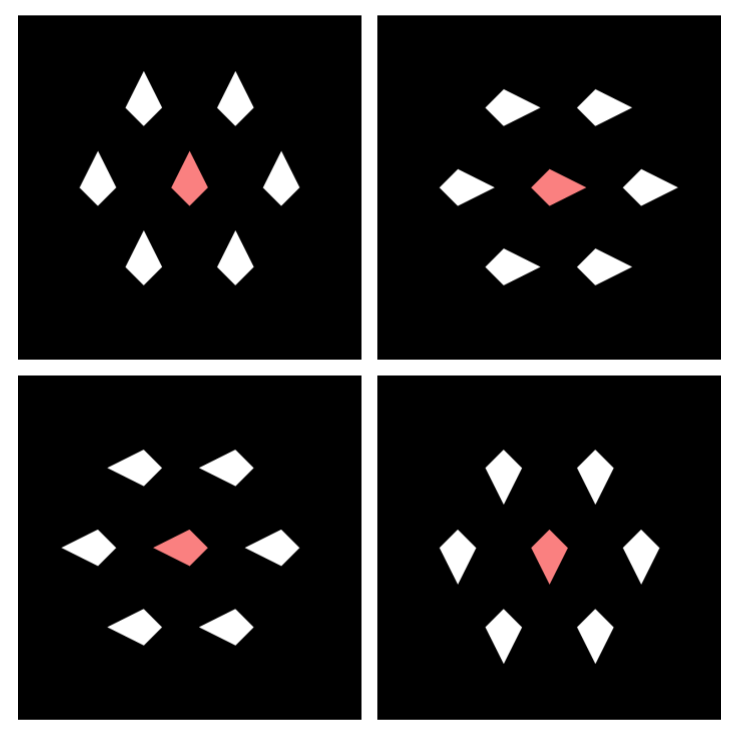
\includegraphics[width=\textwidth]{evoall}
    \caption{The four starting positions we use to evaluate genomes during
    evolution.
    We run the simulation for $100$ steps and calculate the average angle offset
    from the goal direction across the six Reynolds-Vicsek agents.
    The goal direction is east.}
    \label{fig:evo}
\end{figure}
In each of these experiments, the influencing agent is placed in the center of
six Reynolds-Vicsek agents, each of which is at the edge of the influencing
agent's neighborhood.
All agents are initialized to face one of the cardinal directions, and we run
the simulation for $100$ steps.
At the end, we measure the average absolute angle difference, in degrees, from
the goal direction (east) across all six Reynolds-Vicsek agents.
Lower values are better.
Initially, we evaluated genomes during evolution by randomly placing
Reynolds-Vicsek agents in a circle around the influencing agent.
However, random placement resulted in high variability for the same genome
between generations, and it became difficult for the algorithm to find better
genomes.
We ultimately settled on a deterministic test both to reduce this variability
and to allow for memoization to make our algorithm run faster.
Finally, we set our regularization factor $\alpha$ to $0.1$ to allow
development of complexity while also preventing blowout.

\section{Results}
\subsection{No Influencing Agents}

First, we briefly characterize the flocking behavior of a group of Reynolds-Vicsek
agents without influencing agents in the \textit{large} and \textit{herd} settings.
We measure the number of clusters of agents that are path-connected and facing the
same direction; each of these clusters forms a small flock.
We also measure the number of lone agents (the number of agents with no neighbors).
Figure $\ref{fig:no_adhoc}$ shows graphs of these values over time for our two
settings.
\begin{figure}
    \centering
    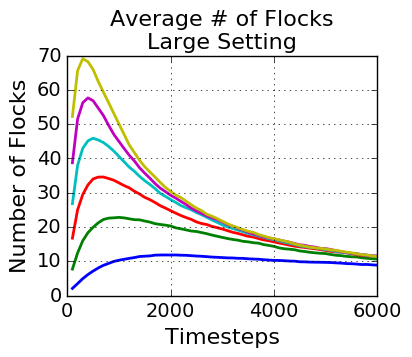
\includegraphics[height=0.33\textwidth]{largeflockNoLegend}
    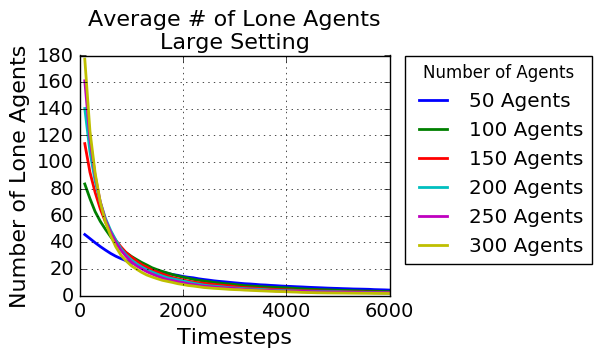
\includegraphics[height=0.33\textwidth]{largeloneWithLegend}
    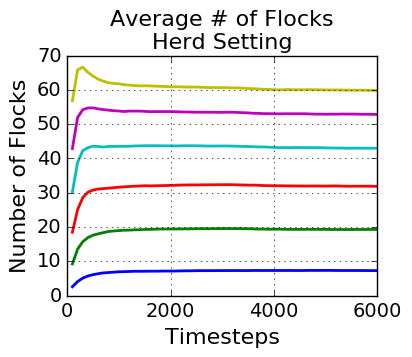
\includegraphics[height=0.33\textwidth]{herdflockNoLegend}
    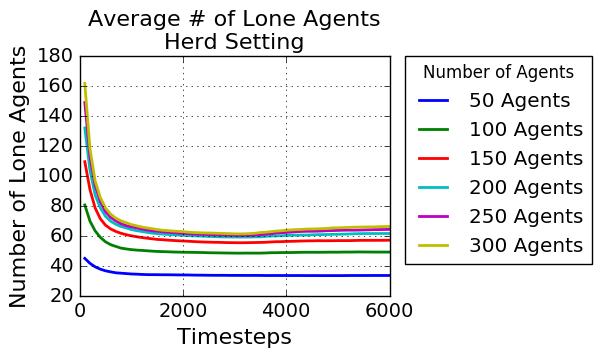
\includegraphics[height=0.33\textwidth]{herdloneWithLegend}
   % \begin{subfigure}[b]{0.24\textwidth}
   %     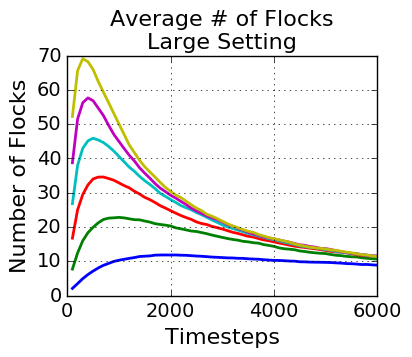
\includegraphics[width=\textwidth]{largeflockNoLegend}
   %     \label{fig:largeflock}
   % \end{subfigure}
   % \begin{subfigure}[b]{0.24\textwidth}
   %     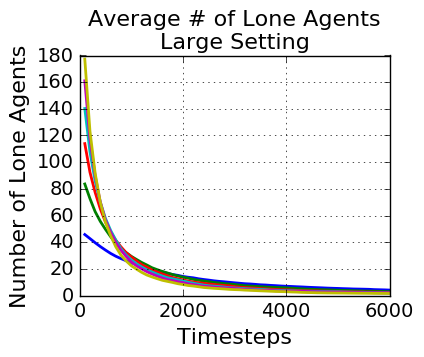
\includegraphics[width=\textwidth]{largeloneNoLegend}
   %     \label{fig:largelone}
   % \end{subfigure}
   % \begin{subfigure}[b]{0.24\textwidth}
   %     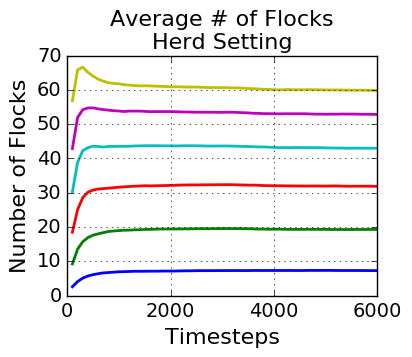
\includegraphics[width=\textwidth]{herdflockNoLegend}
   %     \label{fig:largeflock}
   % \end{subfigure}
   % \begin{subfigure}[b]{0.24\textwidth}
   %     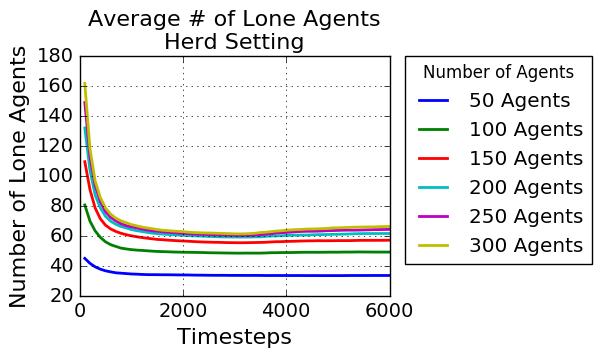
\includegraphics[width=\textwidth]{herdloneWithLegend}
   %     \label{fig:largelone}
   % \end{subfigure}
    \caption{Average flock counts and lone agent counts over time for the
    \textit{large} and \textit{herd} settings with no influencing agents,
    varying the number of Reynolds-Vicsek agents.}
    \label{fig:no_adhoc}
\end{figure}

In the \textit{large} setting, there are two qualitative stages of convergence:
initial flock formation and flock unification.
In the first stage, individual agents collide with each other and form small
flocks, so the number of flocks increases.
In the second stage, these small flocks collide with one another and join
together to form larger flocks, so the number of flocks decreases.
In Figure $\ref{fig:no_adhoc}$, the first stage is represented by the initial
increase in the average number of flocks, and the second stage is represented
by the following decrease in the average number of flocks.
This behavior is reflected in the continually decreasing number of lone agents;
since the number of lone agents continues to decrease over time, we know that the
decrease in the total number of flocks is due to flock convergence.
Note that when there are more total agents, the absolute number of lone agents
decreases faster and reaches a similar value to the other cases by the end of the
simulation.
In other words, the \textit{ratio} of lone agents to total agents hits a
lower value when there are more agents, but the final absolute number of total
lone agents is still similar to the other cases.

The two stages of convergence also occur somewhat in the \textit{herd} setting,
but the second stage is cut off by the non-toroidal nature of the setup.
As flocks leave the starting area, the chances of interacting with other flocks
vastly decreases, so most of the flocks formed from the first stage never end up
merging with other flocks.
This is reflected in the plateaus of both the total number of flocks and the total
number of lone agents.
One small artifact in the metric is worth mentioning: since the agents start
off in a much smaller area than in the \textit{large} setting, many of the
agents start out with a non-zero number of neighbors.
This causes the initial value of the average number of flocks to be non-zero, and
the average number of lone agents to be less than the total number of agents.

\subsection{Influencing Agents in the Large Setting}

Next, we report on the efficacy of the hand-designed behaviors in the
\textit{large} setting.
The average times for $50\%$ convergence with different placement strategies
and our primary six behaviors are shown in Figure $\ref{fig:large}$.
We show graphs for $50$ influencing agents only, since the trends for the other
numbers of influencing agents were similar (the major difference being that
when there are more influencing agents, convergence happens faster).
The results for the \textit{Couzin} behavior are shown at $\omega = 0.5$; this
value was experimentally shown by Couzin et. al. to be the highest value at
this proportion of influencing agents to Reynolds-Vicsek agents that would not
consistently break up the flock.
Note that smaller is better in these graphs.
\begin{figure}
    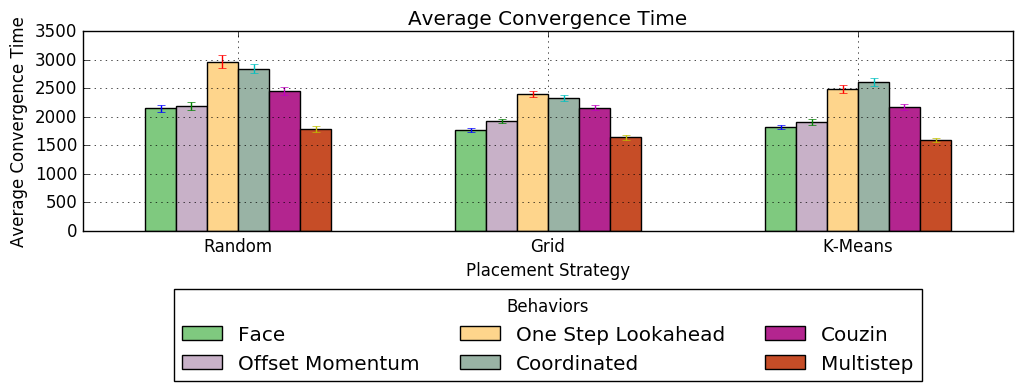
\includegraphics[width=\textwidth]{largesinglerow}
    \caption{Average times to 50\% convergence for $300$ Reynolds-Vicsek agents
    with $50$ influencing agents in the \textit{large} setting under different
    placement strategies and behaviors.
    Smaller is better.
    Error bars show standard error of the mean.}
    \label{fig:large}
\end{figure}

The most immediately striking finding is that, in our more adverse setting,
the \textit{one step lookahead} and \textit{coordinated} behaviors
significantly underperform the ``baseline" \textit{face} and
\textit{offset momentum} behaviors, irrespective of placement strategy.
This is an opposite result from Genter and Stone's findings on smaller simulation
spaces \cite{genter201612steplookahead, genterthesis}, which found that the
\textit{one step lookahead} and \textit{coordinated} behaviors outperform the
\textit{face} and \textit{offset momentum} behaviors.
This finding is also rather counterintuitive; why should the ``smarter" behaviors
underperform the simpler behaviors?

The answer is that, when agent interactions are rare, it is more important for
influencing agents to \textit{maintain influence} than it is for them to quickly
change the direction of neighboring Reynolds-Vicsek agents.
The \textit{one step lookahead} and \textit{coordinated} behaviors underperform
here because they tend to send influencing agents away from neighboring agents.
\begin{figure}
    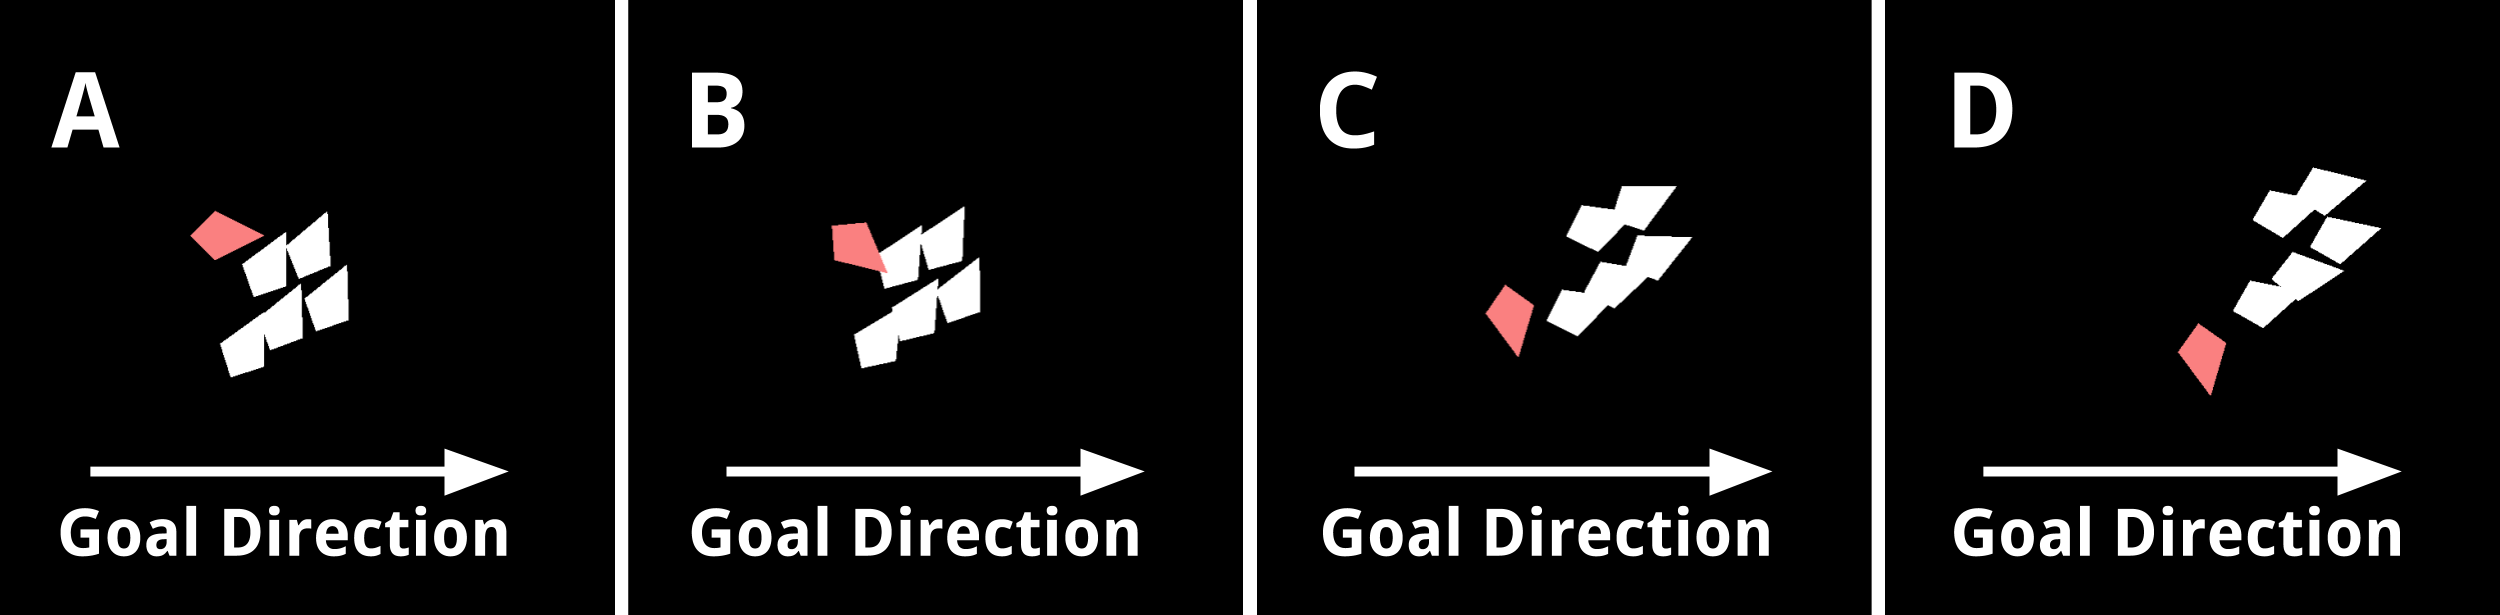
\includegraphics[width=\textwidth]{losing_influence}
    \caption{An example of an influencing agent losing influence under the
    \textit{one step lookahead} behavior.
    The influencing agent is shown in red, and the Reynolds-Vicsek agents are
    shown in white.
    In A, the influencing agent first encounters the flock of Reynolds-Vicsek
    agents.
    In B-D, the influencing agent takes on directions that are oriented away
    from the goal direction to try to rapidly influence the Reynolds-Vicsek
    agents.
    This changes the orientation of the Reynolds-Vicsek agents, but the
    influencing agent has started to travel away from the flock by D.}
    \label{fig:losing_influence}
\end{figure}
An example of this phenomenon is shown in Figure $\ref{fig:losing_influence}$.
The influencing agent, shown in red, adopts an orientation that maximally turns
neighboring Reynolds-Vicsek agents towards the goal direction.
Even though this does turn Reynolds-Vicsek agents towards the goal direction,
it cannot successfully turn all the agents in a single step; as a result, it
must maintain a similar orientation for future steps.
However, as long as the neighboring agents are not facing the goal direction,
the influencing agent's chosen orientation takes it away from the center of the
flock of Reynolds-Vicsek agents, causing it to lose influence.
Once the influencing agent has lost influence, it is difficult to catch up to
the same flock, since influencing agents travel at the same speed\footnote{
There are some approaches that remove this speed constraint from
influencing agents \cite{han2010teleporting}.
However, this allows for unrealistic behaviors wherein influencing agents travel
to one Reynolds-Vicsek agent at a time and change the direction of the
individual Reynolds-Vicsek agent before moving on to the next one.
This results in Reynolds-Vicsek agents that are all facing the same direction,
but that are often not path-connected.}
as Reynolds-Vicsek agents.
As a result, the influencing agent is not actively influencing the direction of
any Reynolds-Vicsek agents until it encounters another group of Reynolds-Vicsek
agents.

Note that this effect also happens on a smaller simulation space, but it is
not nearly as pronounced; when interactions are very frequent, influencing
agents that have lost influence can find another group of Reynolds-Vicsek
agents very quickly.
As a result, the gains from the smarter local algorithm still outweigh the
negative effects from losing influence.

However, it is important to strike a balance between not losing influence and
turning Reynolds-Vicsek agents too slowly.
The \textit{Couzin} algorithm is adept at maintaining influence, but slightly
underperforms the \textit{face} and \textit{offset momentum} behaviors in
measuring time to convergence, because it simply takes longer for influencing
agents to turn the Reynolds-Vicsek agents.

The \textit{multistep} behavior does not suffer from the same problem; it
can both maintain influence and effectively turn Reynolds-Vicsek agents and so
outperforms all the other behaviors by a couple hundred steps (less so under
the \textit{grid} placement strategy).

When the \textit{multistep} behavior is paired with the other behaviors,
it magnifies their inability to maintain influence.
\begin{figure}
    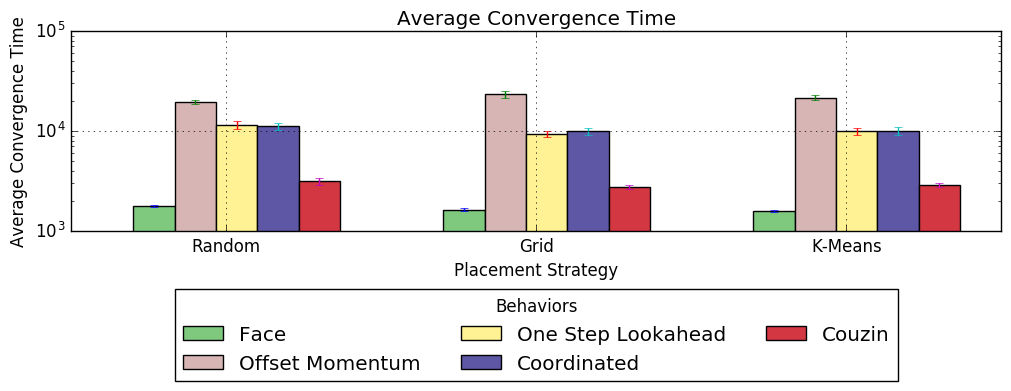
\includegraphics[width=\textwidth]{largesinglerowmultisteplog}
    \caption{Average times to 50\% convergence for $300$ Reynolds-Vicsek agents
    with $50$ influencing agents in the \textit{large} setting under variations
    of the multistep behavior.
    Smaller is better.
    Error bars show standard error of the mean.}
    \label{fig:largemultistep}
\end{figure}
Figure \ref{fig:largemultistep} shows variations on the \textit{multistep}
behavior, wherein influencing agents adopt different behaviors after the number
of Reynolds-Vicsek agents under control passes $T$.
Note that the variations that pair the \textit{multistep} behavior with the
\textit{offset momentum}, \textit{one step lookahead}, and \textit{coordinated}
behaviors perform almost an order of magnitude worse than the vanilla
\textit{multistep} behavior.
What is the root cause of this difference?
The \textit{multistep} behavior starts out by creating many local flocks, some
of which have influencing agents in them.
When interactions are rare, the \textit{offset momentum}, \textit{one step
lookahead}, and \textit{coordinated} behaviors have difficulties changing the
orientation of existing flocks quickly before losing influence.
As a result, the \textit{multistep} behavior takes an order of magnitude longer
to reach convergence when paired with the other behaviors.
This does not happen with the \textit{Couzin} variation of the
\textit{multistep} behavior, since the \textit{Couzin} variation can maintain
influence (note that convergence still takes slightly longer, however).

Finally, we note that the effect of placement behaviors on convergence time
are almost non-existent.
When the density is lower, there is a much smaller chance that any influencing
agent will start out with more than one Reynolds-Vicsek agent in its
neighborhood, even with the \textit{k-means} placement behavior.
As a result, even the best clustering approach is almost the same as starting
out randomly or in a grid.

\subsection{Influencing Agents in the Herd Setting}

Next, we evaluate results for our experiments in the \textit{herd} setting.
In many cases, measuring the number of agents facing the same direction is not
interesting here, since it is impossible to keep Reynolds-Vicsek agents in one place
if they are facing the same direction.
Instead, we exclusively measure the number of Reynolds-Vicsek agents that are
path-connected to influencing agents and facing the same direction as the influencing
agent.
This is a measure of ``control" of the Reynolds-Vicsek agents.
The average number of agents in such local flocks after 15000 time steps is given
in Figure $\ref{fig:herd}$ for both the net and stationary behaviors.
\begin{figure}
    \centering
    \begin{subfigure}[b]{\textwidth}
        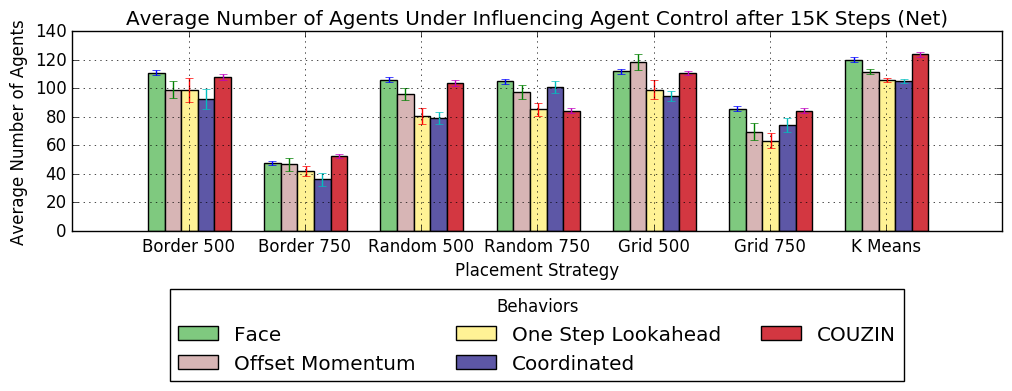
\includegraphics[width=\textwidth]{herd_net}
    \end{subfigure}
    \begin{subfigure}[b]{\textwidth}
        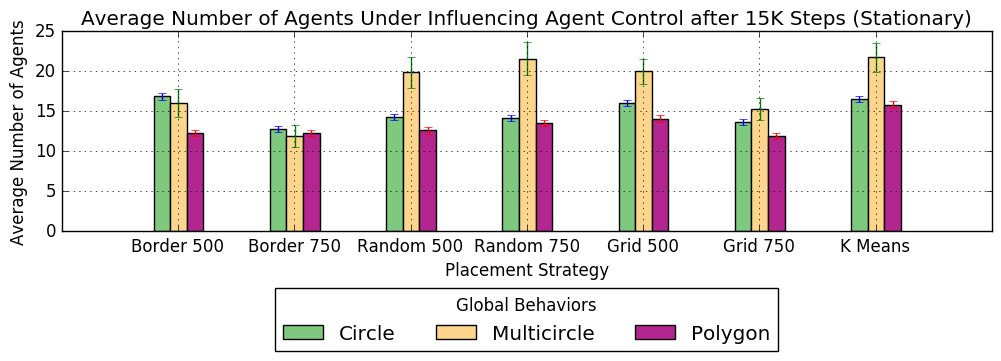
\includegraphics[width=\textwidth]{herd_stationary}
    \end{subfigure}
    \caption{Average number of agents under influencing agent control after $15000$
    steps with $300$ Reynolds-Vicsek agents and $50$ influencing agents in the
    \textit{herd} setting under various placement strategies
    and influencing agent behaviors.
    The net behavior moves the influencing agents and their Reynolds-Vicsek agents
    off-screen, while the stationary behaviors keep the influencing agents near
    the goal area using some sort of circling technique.
    Larger is better.
    Error bars represent standard error of the mean.}
    \label{fig:herd}
\end{figure}
% \begin{figure}
%     \centering
%     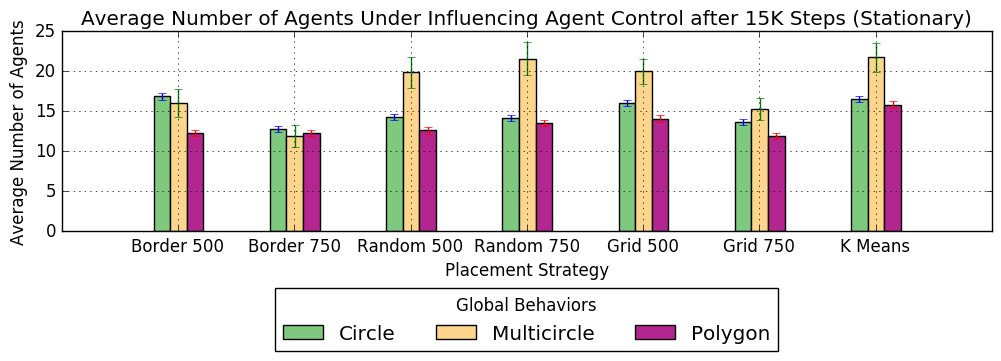
\includegraphics[width=0.50\textwidth]{herd_stationary}
%     \caption{Average number of agents under influencing agent control after $15,000$
%     steps with $300$ Reynolds-Vicsek agents and $50$ influencing agents in the
%     \textit{herd} setting under various stationary behaviors and placement strategies.
%     Stationary behaviors keep the influencing agents near the goal area using some
%     sort of circling technique.
%     For these experiments, we found the only effective local behavior was \textit{face};
%     all the other local behaviors failed to keep Reynolds-Vicsek agents under
%     influencing agent control after $15,000$ steps.
%     Larger is better.}
%     \label{fig:herd_stationary}
% \end{figure}
We find that the net behavior vastly outperforms any of the stationary
behaviors.
However, there may be environments in reality for which the net behavior is not
applicable (suppose it is strictly necessary to keep a flock in one place, for
instance).
Thus, we analyze the net behaviors separately from the stationary behaviors.

\subsubsection{Net}
Again, we find that the \textit{face} behavior tends to outperform the
\textit{offset momentum}, \textit{one step lookahead}, and \textit{coordinated}
behaviors; we attribute this to the tendency of the \textit{offset momentum},
\textit{one step lookahead}, and \textit{coordinated} behaviors to lose
influence over time.
We note that the effect is not as pronounced here as in our \textit{large}
experiments, since each influencing agent has to control fewer agents.
Note that the \textit{face} behavior no longer outperforms the \textit{Couzin}
behavior, except with one placement strategy.
Because the metric has changed to sustained influence over time, it no longer
matters that the \textit{Couzin} behavior turns the Reynolds-Vicsek agents
slower.

In contrast to the \textit{large} experiments, we do find that the placement
strategy has a major effect on the efficacy of the net behavior.
This also has to do with density of influencing agents.
For example, notice that \textit{Border 750} (place the influencing agents in a
circle about the origin with radius $750$) vastly underperforms the other
placement strategies.
The larger radius results in a lower density of influencing agents, so a greater
number of Reynolds-Vicsek agents slip through the ``holes" in the net.
Furthermore, by the time the Reynolds-Vicsek agents reach the border, they have
already formed flocks, and it is more difficult for the influencing agents to
point them in the right direction.
This effect is less pronounced for \textit{Grid 750} and almost non-existent
for \textit{Random 750}, since these strategies place influencing agents within
the circle, and not simply along its circumference.
As a result, the Reynolds-Vicsek agents still encounter influencing agents
before reaching the circumference of the circle.

Finally, we note that \textit{k-means} outperforms all other placement strategies
by a few agents.
Again, the main driving factor behind this is agent density.
When an influencing agent starts out in a clustered area, it has at least one
other Reynolds-Vicsek agent in its neighborhood.
As a result, its effective area of influence is slightly larger than with the
other placement strategies.
This helps it pick up more Reynolds-Vicsek agents in the net.

\subsubsection{Stationary}
For the stationary behaviors, we find that the \textit{multicircle} behavior
slightly underperforms the \textit{circle} behavior when paired with the
\textit{Border} placement strategies; slightly overperforms when paired
with the  \textit{k-means}, \textit{Random}, and \textit{Grid 500} placement
strategies; and performs at par in the \textit{Grid 750} strategy.
What drives these trends?
Once \textit{multicircle} reaches the final stage, it is tracing a larger
circle than the \textit{circle} behavior traces on its own.
As a result, it is easier to maintain influence and turn the Reynolds-Vicsek
agents over time in the final stage.
Before that, however, the influencing agents are in a following stage.
When the influencing agents start out inside the circle, they have more time to
infiltrate small flocks of Reynolds-Vicsek agents and induce a circling
behavior in the final stage.

Finally, we note that \textit{Border 750} is the worst placement strategy,
for reasons similar to the reasons for the net behaviors, and \textit{polygon}
tends to underperform or match the performance of \textit{circle}.
This last observation tells us that adopting occasional sharper turns can
sometimes be harmful, but not always.

\subsection{Evolutionary Experiments}
Next, we report on the results of our evolutionary experiments.
We executed a total of $5$ evolutionary runs.
The first four had population size $25$ and ran for $50$ generations, while the
last one had population size $100$ and ran for $300$ generations.
For the first four runs, we selected the top $10$ genomes to seed the next
generation.
For the last run, we selected the top $20$ genomes.
As an optimization, we memoized genomes from generation to generation and re-used
results where possible.
We allowed for duplicate members in the population.
The average angle difference across the population and the angle difference of
the best genome in each generation are shown in Figure $\ref{fig:genetic_runs}$.
We also show performances of the \textit{face}, \textit{offset momentum},
\textit{one step lookahead}, and \textit{Couzin} behaviors for comparison.
We do not show the \textit{coordinated} behavior, since it is equivalent
to the \textit{one step lookahead} behavior when there is only a single
influencing agent.
\begin{figure}
    \centering
    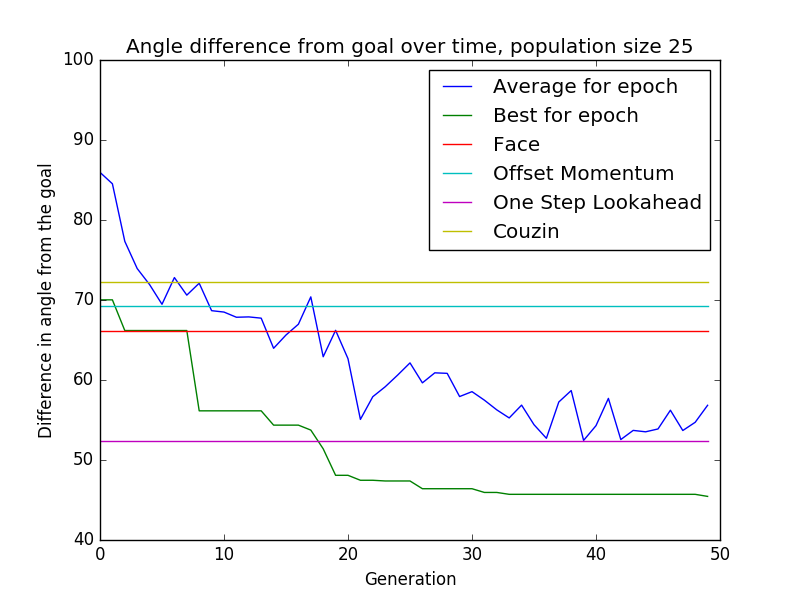
\includegraphics[width=0.45\textwidth]{run07}
    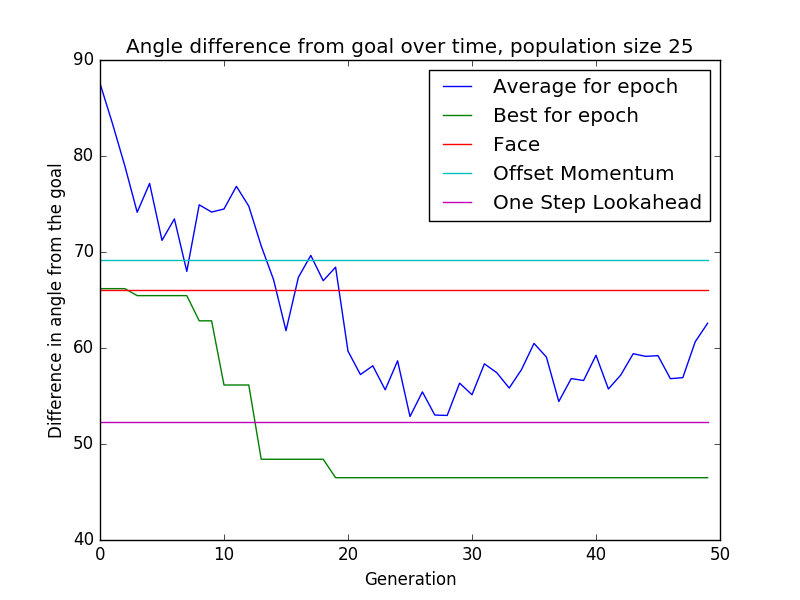
\includegraphics[width=0.45\textwidth]{run08}
    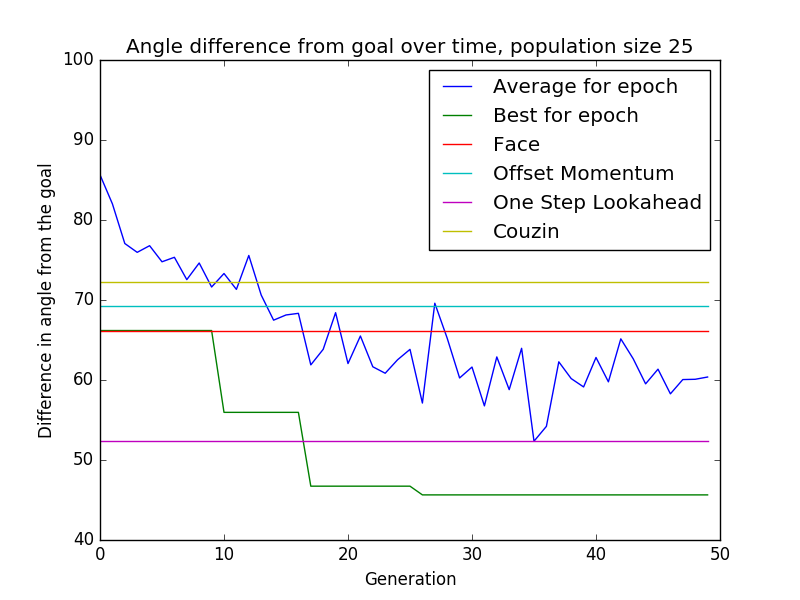
\includegraphics[width=0.45\textwidth]{run09}
    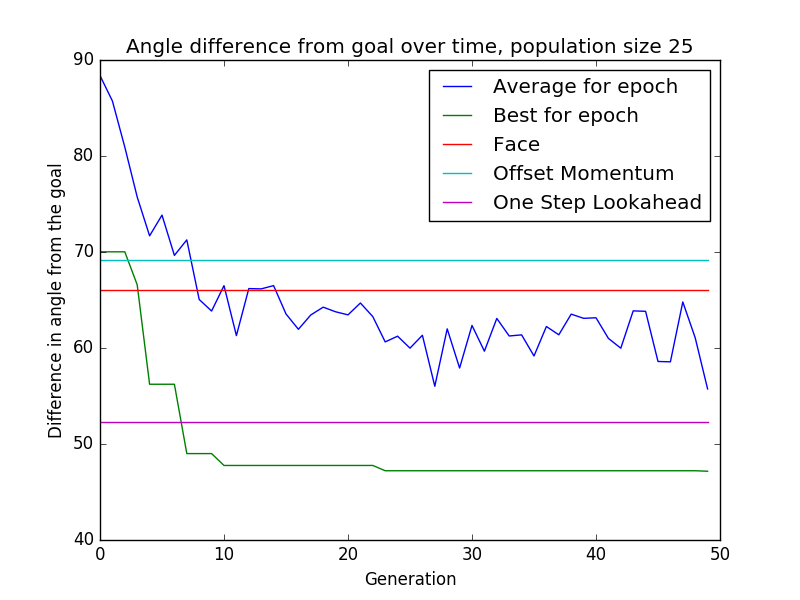
\includegraphics[width=0.45\textwidth]{run10}
    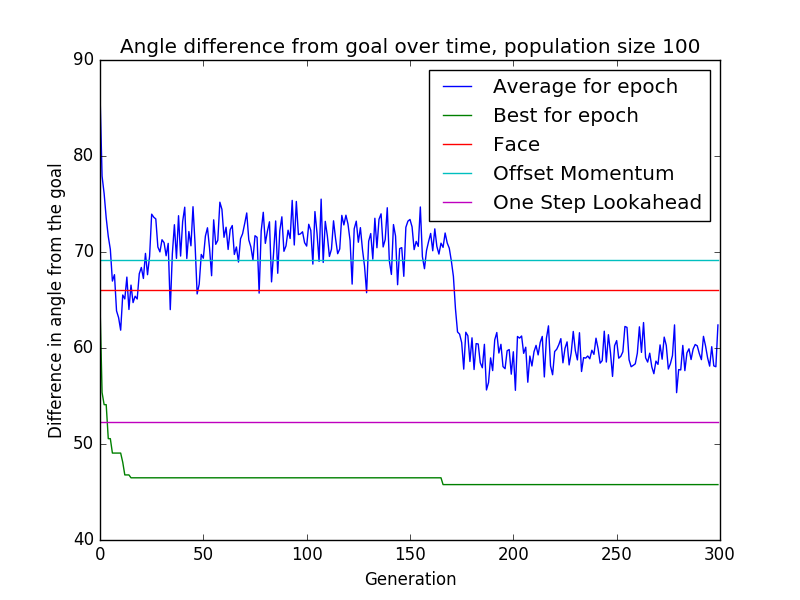
\includegraphics[width=0.45\textwidth]{run11}
    \caption{Average population fitness and fitness of the best candidate in the
    population over generations for a five different runs of the genetic algorithm.
    The first four runs had population size $25$ and ran for $50$ generations,
    while the last run has population size $100$ and ran for $300$ generations.
    Fitnesses of the \textit{face}, \textit{offset momentum}, \textit{one step
    lookahead}, and \textit{Couzin} behaviors provided for comparison.}
    \label{fig:genetic_runs}
\end{figure}

In each run, the population converged to one or two best genomes that remained
in the seed population for every generation.
These best genomes consistently outperformed the hand-constructed behaviors
taken from the literature.
However, the average angle difference across the population stayed relatively
high throughout the entire simulation, since the majority of the population
was the result of random mutation or crossover from the seed population.
In many cases, the new children perform very poorly, driving the average angle
difference up.
In the last run, with a population of size $100$, there is a sharp drop in the
average angle difference around generation $160$.
At this point in the evolutionary run, a single genome out-competed all the
others.
As a result, all subsequent populations were seeded by multiple copies of a
single genome, and mutations/crossover performed on this seed population
were relatively stable.

From these five evolutionary runs, we selected $7$ for further analysis.
These are shown in Table $\ref{table:genomes}$
\begin{table}[h]
\centering
\begin{tabular}{|c|c|}
    \hline
    \textbf{Name} & \textbf{Genome} \\
    \hline
    \multirow{2}{*}{G1} & acc=goal; (mul acc (gez (cos heading) \\
        & (exp (sin heading) distance) (sin goal))) \\ \hline
    G2 & acc=goal; (mul influence (mul influence goal)) \\ \hline
    G3 & acc=goal; (sub acc (mul -0.2678771899171444 goal)) \\ \hline
    G4 & acc=goal; (mul (mul acc (cos heading)) distance) \\ \hline
    \multirow{3}{*}{G5} & acc=goal; (mul distance \\
    &(mul (sub (sub goal 0.2801770623593902) heading) \\
    & (mul (sub acc heading) goal))) \\ \hline
    \multirow{3}{*}{G6} & acc=goal; (mul distance (mul (sin influence) \\
    & (mul (sub (sub goal 0.2801770623593902) heading) \\
    & (mul (sub (sub goal 0.2801770623593902) heading) goal)))) \\ \hline
    G7 & acc=goal; (mul goal (gez (cos acc) 0.19745673470999736 goal)) \\ \hline
\end{tabular}
\caption{Genomes from evolution}
\label{table:genomes}
\end{table}
These genomes bear a few similarities to each other; they all initialize the
accumulator to the goal direction, for example.
Beyond that, they share very little in common.
Some genomes (G1, G3, G5, G7) use the accumulator, while the others do not; some
are short and easy to parse (G2 is equivalent to $\frac{goal}{N^2}$, where
$N$ is the number of neighbors), while others are much more complicated.

Although they may be very different in expression, they are very similar to each
other in execution.
When all the agents are already facing east, these behaviors all have the
influencing agent face east as well.
In addition, they pick up some gains from the north and south starting conditions
by initially picking up more neighbors than the baseline conditions.
They pick up some major gains in the west case, where they intersect a few of
the neighbors behind them and lead them towards the target direction over the
course of the next $100$ steps.
A few screenshots of this process are shown in Figure $\ref{fig:g1}$.
\begin{figure}
    \centering
    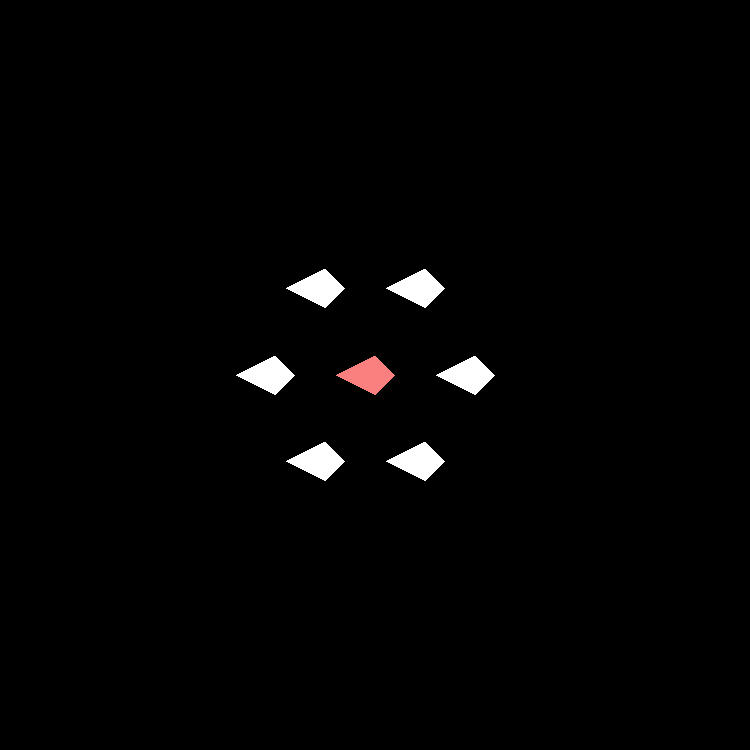
\includegraphics[width=0.32\textwidth]{westgenetic01}
    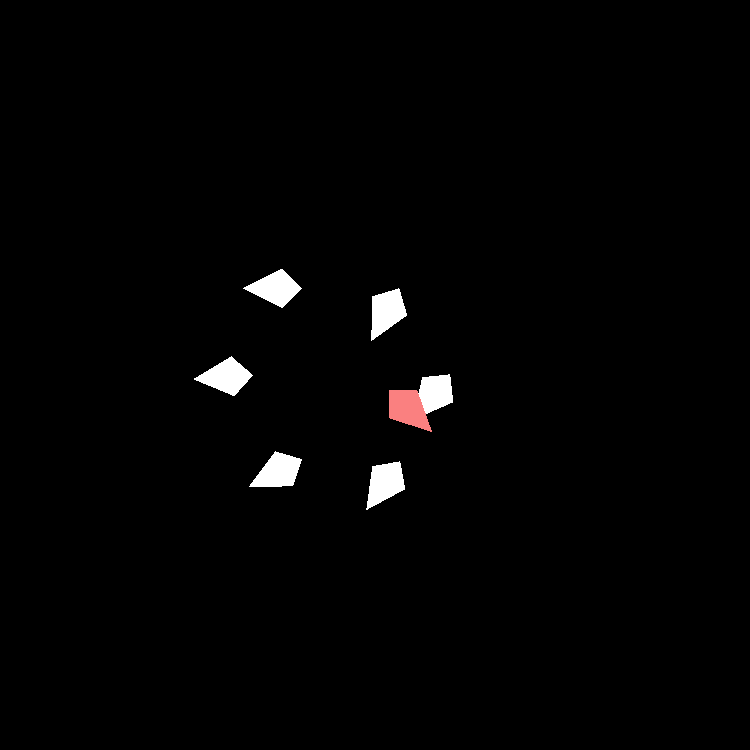
\includegraphics[width=0.32\textwidth]{westgenetic02}
    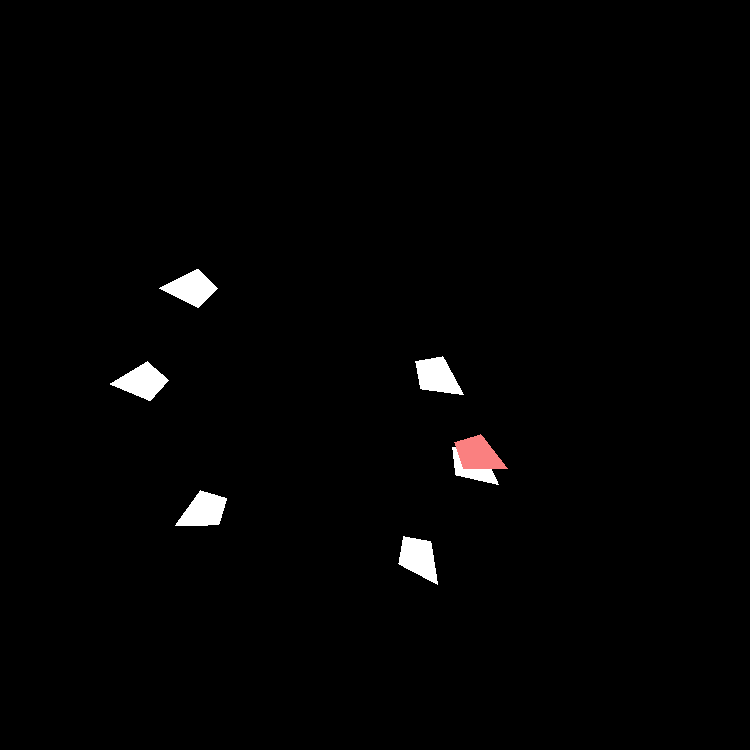
\includegraphics[width=0.32\textwidth]{westgenetic03}
    \caption{Screenshots of the G1 behavior when trying to turn $6$
    Reynolds-Vicsek agents $180$ degrees to the east.
    Instead of trying to turn all $6$ neighbors at once, as the \textit{one step
    lookahead} behavior does, the genetic behavior ``gives up" on some neighbors
    and just tries to turn the neighbors that are behind it.}
    \label{fig:g1}
\end{figure}
The other genetic processes behave very similarly to the behavior shown in the
screenshots, with slight variations (i.e., turning north instead of south, etc).

This behavior is very interesting scientifically for the differences between it
and the \textit{one step lookahead} behavior.
In particular, the genetic behaviors immediately turn towards the Reynolds-Vicsek
agents behind them, and ignore the agents in front of them.
There are two major insights we can glean from this behavior.
First, when the influencing agents focus on the agents behind them, they can
successfully maintain influence over time instead of flying away from the flock
as they try to turn their neighbors towards the goal direction.
In other words, the genetic behaviors implicitly value influence over rapid
convergence.
We hypothesize that this arises because evaluation happens after $100$ steps and
not after $1$ step, as with the \textit{one step lookahead} behavior, but more
work is needed to answer this definitively.

Second, the influencing agents ignore the Reynolds-Vicsek agents in front of
them.
There are a few reasons why this is beneficial.
Since the influencing agents have limited speed, they can never ``catch
up" to the agents directly in front of them.
The \textit{one step lookahead} behavior does not take this into account;
as long as a neighbor is in range, its heading is factored into the calculation,
no matter whether the influencing agent can ever reach the neighbor.
Furthermore, it is much easier to lose influence over forward neighbors, since
any change in direction necessarily means that the influencing agent falls
behind.
Thus, the Reynolds-Vicsek agents in front are somewhat of a lost cause, and it
is beneficial to ignore them.

\subsection{Influencing Agents in the Large and Herd Settings}
Next, we verify that the genetic algorithms are still effective when used in
our larger settings.
For example, the \textit{one step lookahead} behavior outperforms the
\textit{face} behavior in the small-scale evaluations we use during evolution,
but underperforms the \textit{face} behavior in the \textit{large} setting.
The results are shown in Figure $\ref{fig:largegenetic}$.

\begin{figure}
    \centering
    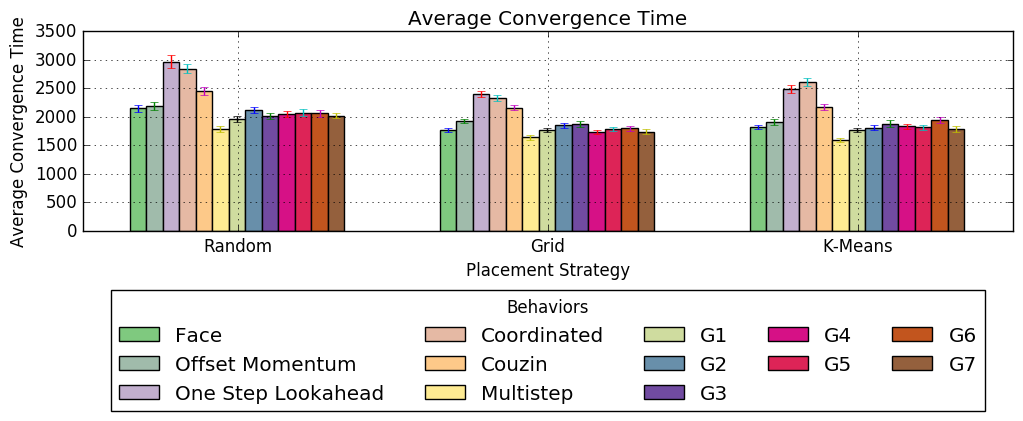
\includegraphics[width=\textwidth]{largegeneticsinglerow}
    \caption{Average times to 50\% convergence for $300$ Reynolds-Vicsek agents
    with $50$ influencing agents in the \textit{large} setting under different
    placement strategies, paired with our hand-designed behaviors and the
    selected genetic behaviors.
    Smaller is better.
    Error bars show standard error of the mean.}
    \label{fig:largegenetic}
\end{figure}
We find that these genetic behaviors all perform on par with, or slightly
better than, the \textit{face} behavior.
They all strongly outperform the \textit{one step lookahead} and
\textit{coordinated} behaviors, and slightly outperform the
\textit{offset momentum} behavior.
None perform as well as the \textit{multistep} behavior.

%When paired with the \textit{random} global behavior, however, the story changes
%drastically.
%Genetic behaviors G1, G4, and G7 still perform on par with the \textit{face} local
%behavior, but G2, G3, and G6 start performing as poorly as \textit{one step
%lookahead}.
%G5 takes a major hit; instead of converging within $4000$ timesteps, it takes up to
%$30000$ timesteps to converge.
%From watching the simulations, a very peculiar behavior emerges: when the
%influencing agent is moving in a random direction and meets a flock moving in a
%similar direction, the agent continues moving in the direction of the flock
%instead of turning the flock towards the goal direction.
%It is not clear to us why this behavior emerges, especially since G5's genome
%is one of the harder genomes to parse.
%
%When paired with the \textit{multistep} global behavior, G1-3 once again
%perform on par with the \textit{face} local behavior.
%The G5 behavior again performs much worse, and the G6 behavior performs slightly
%worse than the \textit{face} local behavior.
%G4 and G7 perform slightly better than G1-3, and slightly outperform \textit{face}
%(though not by a significant amount).
%Notably, none of the genetic behaviors, not even G5, perform as badly as \textit{
%offset momentum} and \textit{one step lookahead} do when paired with the
%\textit{multistep} global behavior.
%This is promising; it suggests that there are behaviors that can be more effective
%than \textit{face} on a small scale but that can remain effective even when moving
%to low-density settings.

%\subsection{Influencing Agents in the Herd Setting}

Figure \ref{fig:herdnetgenetic} shows the performance of the genetic algorithms
when used in the \textit{net} case of the \textit{herd} setting.
\begin{figure}
    \centering
    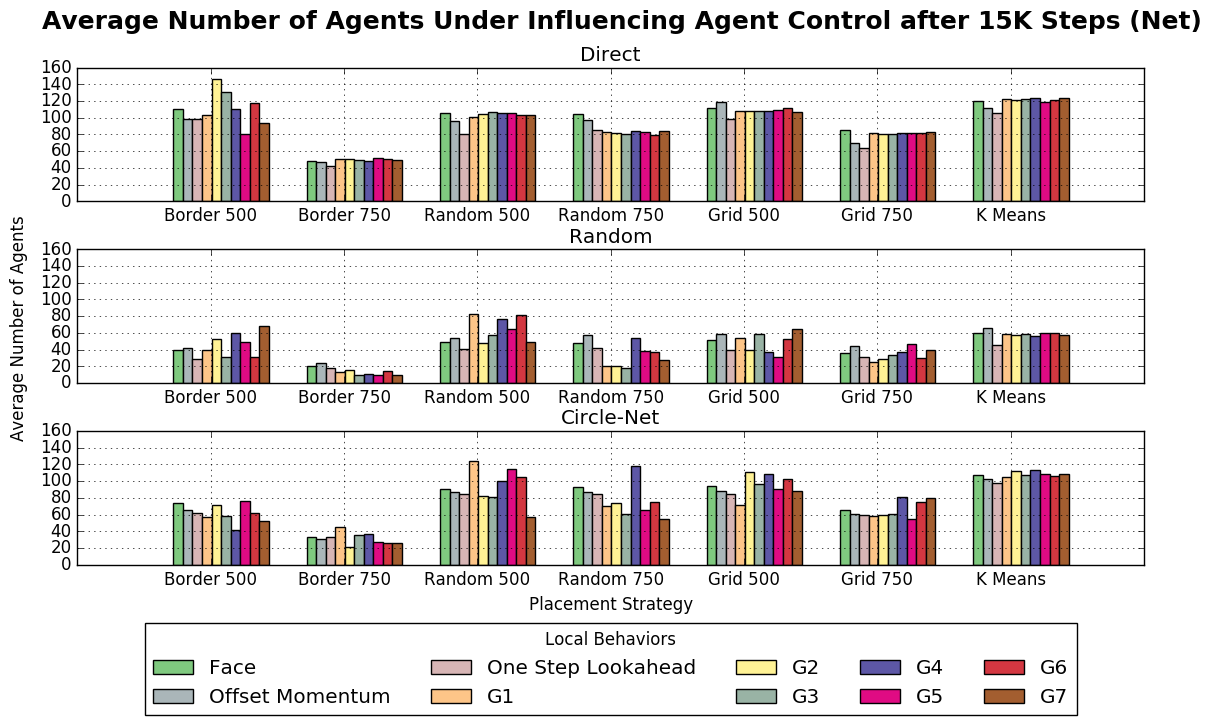
\includegraphics[width=\textwidth]{herd_net_genetic}
    \caption{Average number of agents under influencing agent control after $15000$
    steps with $300$ Reynolds-Vicsek agents and $50$ influencing agents in the
    \textit{herd} setting under for various placement strategies and behaviors,
    including the genetic algorithms.
    Larger is better.
    Error bars show standard error of the mean.}
    \label{fig:herdnetgenetic}
\end{figure}
Again, across the board, the genetic behaviors perform as well as the
\textit{face} and \textit{Couzin} behaviors, and outperform the \textit{offset
momentum}, \textit{one step lookahead}, and \textit{coordinated} behaviors.
The only exception is in the \textit{Random 750} placement strategy, where all
the genetic behaviors do worse.
We are not sure what drives this effect, but we note that the \textit{Couzin}
strategy also performs poorly with this placement strategy; these results may
be related in some way.
